\PassOptionsToPackage{unicode=true}{hyperref} % options for packages loaded elsewhere
\PassOptionsToPackage{hyphens}{url}
%
\documentclass[
  ignorenonframetext,
]{beamer}
\usepackage{pgfpages}
\setbeamertemplate{caption}[numbered]
\setbeamertemplate{caption label separator}{: }
\setbeamercolor{caption name}{fg=normal text.fg}
\beamertemplatenavigationsymbolsempty
% Prevent slide breaks in the middle of a paragraph:
\widowpenalties 1 10000
\raggedbottom
\setbeamertemplate{part page}{
  \centering
  \begin{beamercolorbox}[sep=16pt,center]{part title}
    \usebeamerfont{part title}\insertpart\par
  \end{beamercolorbox}
}
\setbeamertemplate{section page}{
  \centering
  \begin{beamercolorbox}[sep=12pt,center]{part title}
    \usebeamerfont{section title}\insertsection\par
  \end{beamercolorbox}
}
\setbeamertemplate{subsection page}{
  \centering
  \begin{beamercolorbox}[sep=8pt,center]{part title}
    \usebeamerfont{subsection title}\insertsubsection\par
  \end{beamercolorbox}
}
\AtBeginPart{
  \frame{\partpage}
}
\AtBeginSection{
  \ifbibliography
  \else
    \frame{\sectionpage}
  \fi
}
\AtBeginSubsection{
  \frame{\subsectionpage}
}
\usepackage{lmodern}
\usepackage{amssymb,amsmath}
\usepackage{ifxetex,ifluatex}
\ifnum 0\ifxetex 1\fi\ifluatex 1\fi=0 % if pdftex
  \usepackage[T1]{fontenc}
  \usepackage[utf8]{inputenc}
  \usepackage{textcomp} % provides euro and other symbols
\else % if luatex or xelatex
  \usepackage{unicode-math}
  \defaultfontfeatures{Scale=MatchLowercase}
  \defaultfontfeatures[\rmfamily]{Ligatures=TeX,Scale=1}
\fi
% use upquote if available, for straight quotes in verbatim environments
\IfFileExists{upquote.sty}{\usepackage{upquote}}{}
\IfFileExists{microtype.sty}{% use microtype if available
  \usepackage[]{microtype}
  \UseMicrotypeSet[protrusion]{basicmath} % disable protrusion for tt fonts
}{}
\makeatletter
\@ifundefined{KOMAClassName}{% if non-KOMA class
  \IfFileExists{parskip.sty}{%
    \usepackage{parskip}
  }{% else
    \setlength{\parindent}{0pt}
    \setlength{\parskip}{6pt plus 2pt minus 1pt}}
}{% if KOMA class
  \KOMAoptions{parskip=half}}
\makeatother
\usepackage{xcolor}
\IfFileExists{xurl.sty}{\usepackage{xurl}}{} % add URL line breaks if available
\IfFileExists{bookmark.sty}{\usepackage{bookmark}}{\usepackage{hyperref}}
\hypersetup{
  pdftitle={Bayesian design and analysis of external pilot trials for complex interventions},
  pdfauthor={Duncan T. Wilson},
  pdfborder={0 0 0},
  breaklinks=true}
\urlstyle{same}  % don't use monospace font for urls
\newif\ifbibliography
\setlength{\emergencystretch}{3em}  % prevent overfull lines
\providecommand{\tightlist}{%
  \setlength{\itemsep}{0pt}\setlength{\parskip}{0pt}}
\setcounter{secnumdepth}{-2}

% set default figure placement to htbp
\makeatletter
\def\fps@figure{htbp}
\makeatother


\title{Bayesian design and analysis of external pilot trials for complex
interventions}
\author{Duncan T. Wilson}
\date{November 14, 2018}

\begin{document}
\frame{\titlepage}

\hypertarget{background}{%
\section{Background}\label{background}}

\begin{frame}{External pilot trials}
\protect\hypertarget{external-pilot-trials}{}

\(\{\text{Pilot trials}\} \subset \{\text{Feasibility studies}\}\)
(Eldridge et al. 2016)

A small version of the planned main study

Asking the questions: \emph{should} we do the main trial, and if so,
\emph{how}?

Common quantitative objectives: estimating recruitment rates, follow-up
rates, and adherence rates (Avery et al. 2017)

\end{frame}

\begin{frame}{Designing pilot trials}
\protect\hypertarget{designing-pilot-trials}{}

Sample size is often a rule-of-thumb: 12, 30, 35 patients per arm

Methods almost always motivated by estimating a standard deviation
nuisance parameter

Very little looking at other objectives, like estimating a rate. Some
methods based on precision (Eldridge et al. 2015), or a Bayesian
approach (Hampson et al. 2017)

\end{frame}

\begin{frame}{Analysing pilot trials}
\protect\hypertarget{analysing-pilot-trials}{}

Analyse the pilot data to decide if the definitive trial should go ahead
- base the decision on \emph{progression criteria}. For example,

\begin{itemize}
\tightlist
\item
  Recruit at least 40\% of residents in each care home
\item
  Have no more than 60\% loss to follow-up
\item
  At least 50\% of participants attend 8 or more therapy sessions
\end{itemize}

Can also be ``traffic lights'' - red (stop), green (go), amber (modify)

Effectiveness rarely assessed - concerns of low power

Little guidance available on how to choose thresholds

Statistical nature of the problem often ignored

\end{frame}

\begin{frame}{Progression criteria}
\protect\hypertarget{progression-criteria}{}

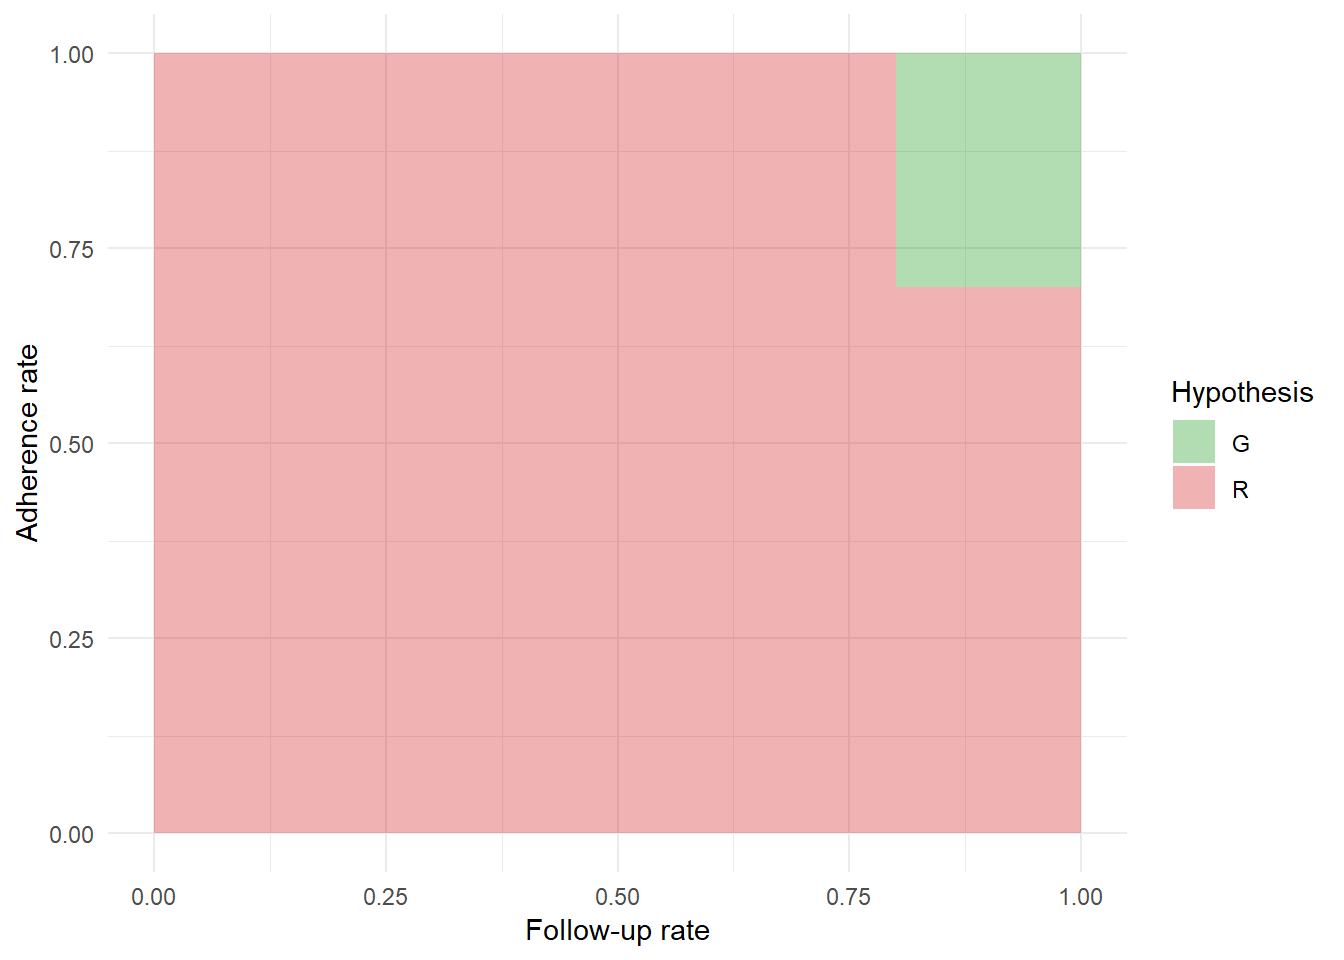
\includegraphics[width=0.9\linewidth,height=0.7\textheight]{Bayes_pilot_pres_files/figure-beamer/unnamed-chunk-1-1}

\end{frame}

\begin{frame}{Motivation}
\protect\hypertarget{motivation}{}

Several outcomes, hard/impossible to balance trade-offs

Complex models with unknown nuisance parameters, e.g.~an ICC in a cRCT

Bayesian approch can deal with both of these

Questions:

\begin{itemize}
\tightlist
\item
  How should we make progression decisions after a Bayesain analysis?
\item
  How can we evaluate a Bayesain pilot design and choose its sample
  size?
\end{itemize}

\end{frame}

\hypertarget{methods}{%
\section{Methods}\label{methods}}

\begin{frame}{Hypotheses}
\protect\hypertarget{hypotheses}{}

Identify anreas of the parameter space where we would ideally like to
\emph{stop} (R), \emph{modify} (A), or \emph{go} (G):

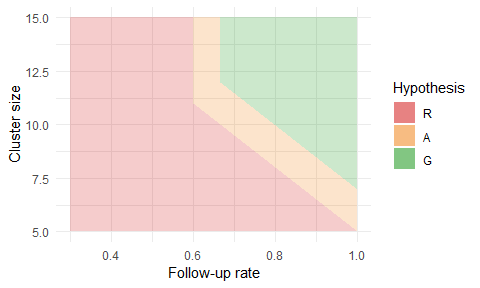
\includegraphics[width=0.9\linewidth,height=0.7\textheight]{Bayes_pilot_pres_files/figure-beamer/unnamed-chunk-2-1}

\end{frame}

\begin{frame}{Loss}
\protect\hypertarget{loss}{}

\begin{table}
\caption{Losses associated with each decision under each hypothesis.}
\centering
\begin{tabular}{r r c c c}
\toprule
& & \multicolumn{3}{c}{Hypothesis} \\
& & $\phi \in \Phi_{R}$ & $\phi \in \Phi_{A}$ & $\phi \in \Phi_{G}$ \\
\midrule
\multirow{3}{*}{Decision} & $r$ & 0 & $c_{2}$ & $c_{2}$ \\
 & $a$ & $c_{1} + c_{3}$ & 0 & $c_{3}$ \\
 & $g$ & $c_{1}$ & $c_{1} + c_{2}$ & 0  \\
\bottomrule
\end{tabular}
\label{tab:loss}
\end{table}

Three types of errors:

\begin{itemize}
\tightlist
\item
  \(E_1\): proceeding to a futile trial
\item
  \(E_2\): discarding a promising intervention
\item
  \(E_3\): needlessly modifying the intervention or trial design
\end{itemize}

\[
L(d, \phi) = c_1 E_1(d, \phi) + c_2 E_2(d, \phi) + c_3 E_3(d, \phi).
\]

\end{frame}

\begin{frame}{Expected loss}
\protect\hypertarget{expected-loss}{}

After seeing the pilot data \(x\), we choose the action with the best
expected loss:

\[
\begin{align}
i^{*} & = \arg\min_{i \in \{r,a,g\}} \mathbb{E}_{\phi | x} [ L(i, \phi) ] \\
 & = \arg\min_{i \in \{r,a,g\}} \int L(i, \phi) p(\phi | x) d\phi.
\end{align}
\] Let \(p_I\) be the posterior probability of hypothesis \(I\), given
the pilot data. Then,

\[
\begin{aligned}
\mathbb{E}_{\phi | x} [ L(r, \phi) ] & = p_{A}c_{3} + p_{G}c_{3}, \\
\mathbb{E}_{\phi | x} [ L(a, \phi) ] & = p_{R}c_{1} + p_{R}c_{2} + p_{G}c_{2}, \\
\mathbb{E}_{\phi | x} [ L(g, \phi) ] & = p_{R}c_{1} + p_{A}c_{1} + p_{A}c_{3}.
\end{aligned}
\]

\end{frame}

\begin{frame}{Operating characteristics and optimisation}
\protect\hypertarget{operating-characteristics-and-optimisation}{}

Operating characteristics:

\begin{itemize}
\tightlist
\item
  \(OC_1 = Pr[a ~\&~ \phi \in \Phi_R] + Pr[g ~\&~ \phi \in \Phi_R \cup \Phi_A]\)
  - probability of proceeding to a futile main RCT;
\item
  \(OC_2 = Pr[r ~\&~ \phi \in \Phi_A \cup \Phi_G] + Pr[g ~\&~ \phi \in \Phi_A]\)
  - probability of discarding a promising intervention;
\item
  \(OC_3 = Pr[a ~\&~ \phi \in \Phi_R \cup \Phi_G]\) - probability of
  making unnecessary adjustments to the intervention or the trial
  design.
\end{itemize}

\end{frame}

\begin{frame}{Operating characteristics and optimisation}
\protect\hypertarget{operating-characteristics-and-optimisation-1}{}

Solve the multi-objective optimisation problem \[
\min_{\mathbf{c} \in \mathcal{C}} ~ \left( OC_{1}(\mathbf{c}),~ OC_{2}(\mathbf{c}),~ OC_{3}(\mathbf{c}) \right)
\] where
\(\mathcal{C} = \{c_{1}, c_{2} \in [0,1] ~|~ c_{1} + c_{2} \leq 1\}\).

\(\rightarrow\) a set of options for the cost parameters, offering
different trade-offs between the three operating characteristics

\end{frame}

\hypertarget{illustrative-application}{%
\section{Illustrative application}\label{illustrative-application}}

\begin{frame}{REACH}
\protect\hypertarget{reach}{}

REACH (Research Exploring Physical Activity in Care Homes): a pilot for
a complex intervention designed to increase the physical activity of
care home residents

Feasibility outcomes:

\begin{itemize}
\tightlist
\item
  recruitment (measured in terms of the average number of residents in
  each care home who participate in the trial);
\item
  adherence (a binary indicator at the care home level indicating if the
  intervention was fully implemented);
\item
  data completion (a binary indicator for each resident of successful
  follow-up at the planned primary outcome time of 12 months);
\item
  efficacy (a continuous measure of physical activity at the resident
  level).
\end{itemize}

\end{frame}

\begin{frame}{Hypotheses}
\protect\hypertarget{hypotheses-1}{}

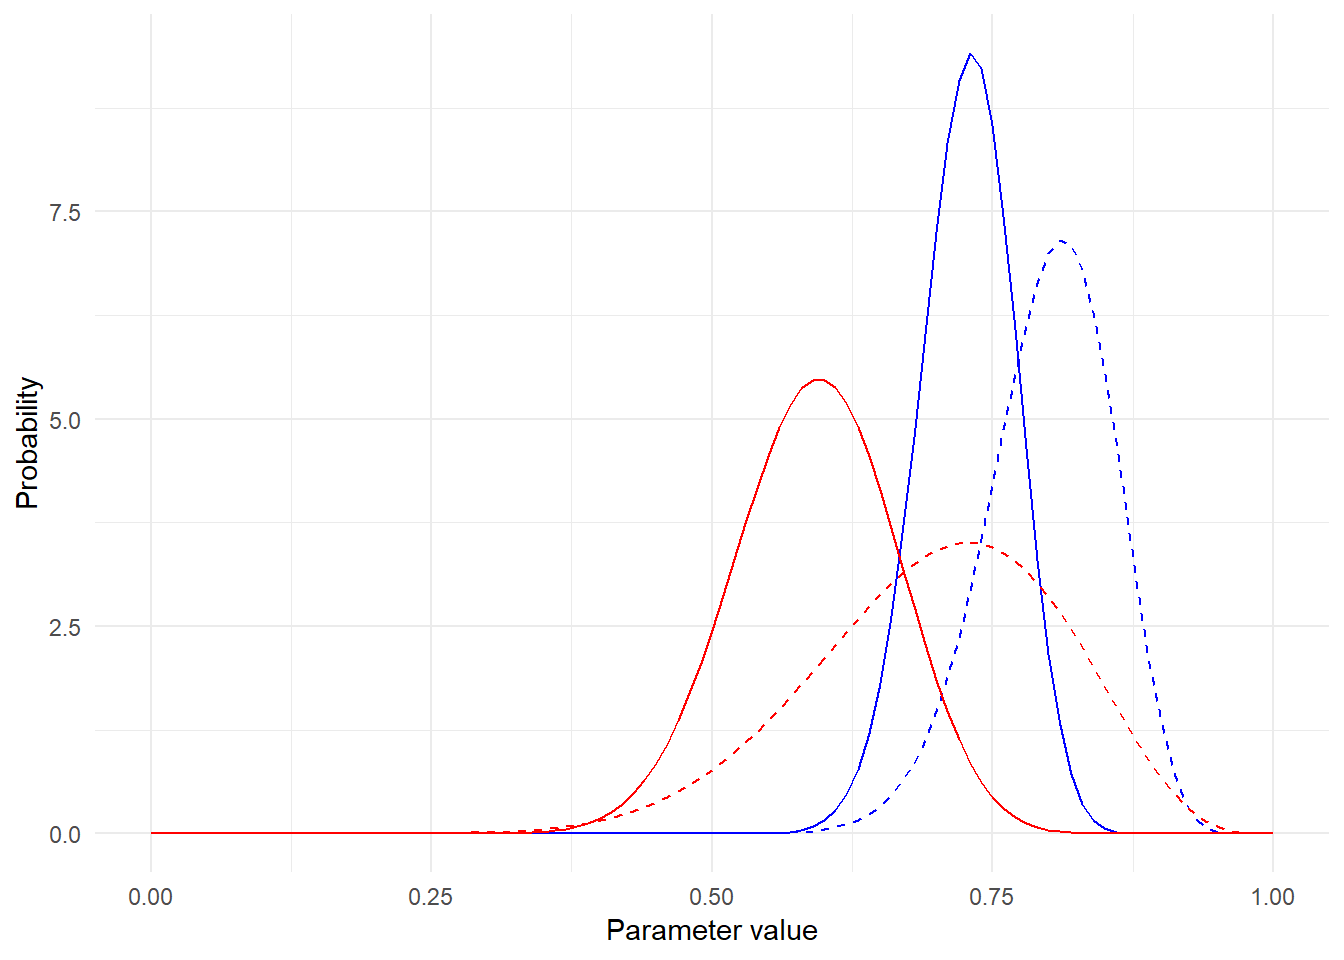
\includegraphics[width=0.9\linewidth,height=0.7\textheight]{Bayes_pilot_pres_files/figure-beamer/unnamed-chunk-3-1}

\end{frame}

\begin{frame}{Hypotheses}
\protect\hypertarget{hypotheses-2}{}

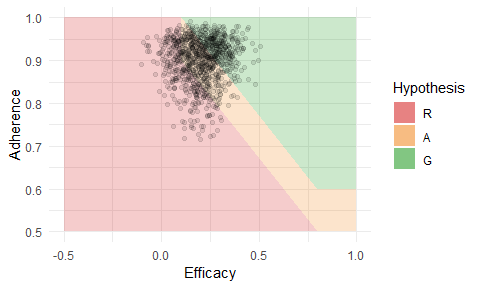
\includegraphics[width=0.9\linewidth,height=0.7\textheight]{Bayes_pilot_pres_files/figure-beamer/unnamed-chunk-4-1}

\end{frame}

\begin{frame}[fragile]{Optimisation}
\protect\hypertarget{optimisation}{}

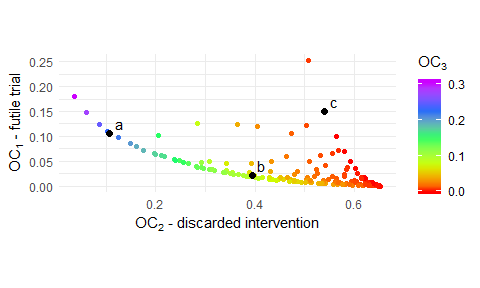
\includegraphics[width=0.9\linewidth,height=0.7\textheight]{Bayes_pilot_pres_files/figure-beamer/unnamed-chunk-5-1}

\begin{verbatim}
##     Label  $(c_1, c_2, c_3)$        $OC_1$        $OC_2$        $OC_3$
## 96      a  (0.07, 0.03, 0.9) 0.107 (0.003) 0.108 (0.003) 0.232 (0.004)
## 49      b (0.18, 0.24, 0.58) 0.021 (0.001) 0.394 (0.005)  0.08 (0.003)
## 275     c  (0.01, 0.7, 0.29) 0.151 (0.004) 0.539 (0.005)     0.002 (0)
\end{verbatim}

\end{frame}

\begin{frame}{Subjective priors}
\protect\hypertarget{subjective-priors}{}

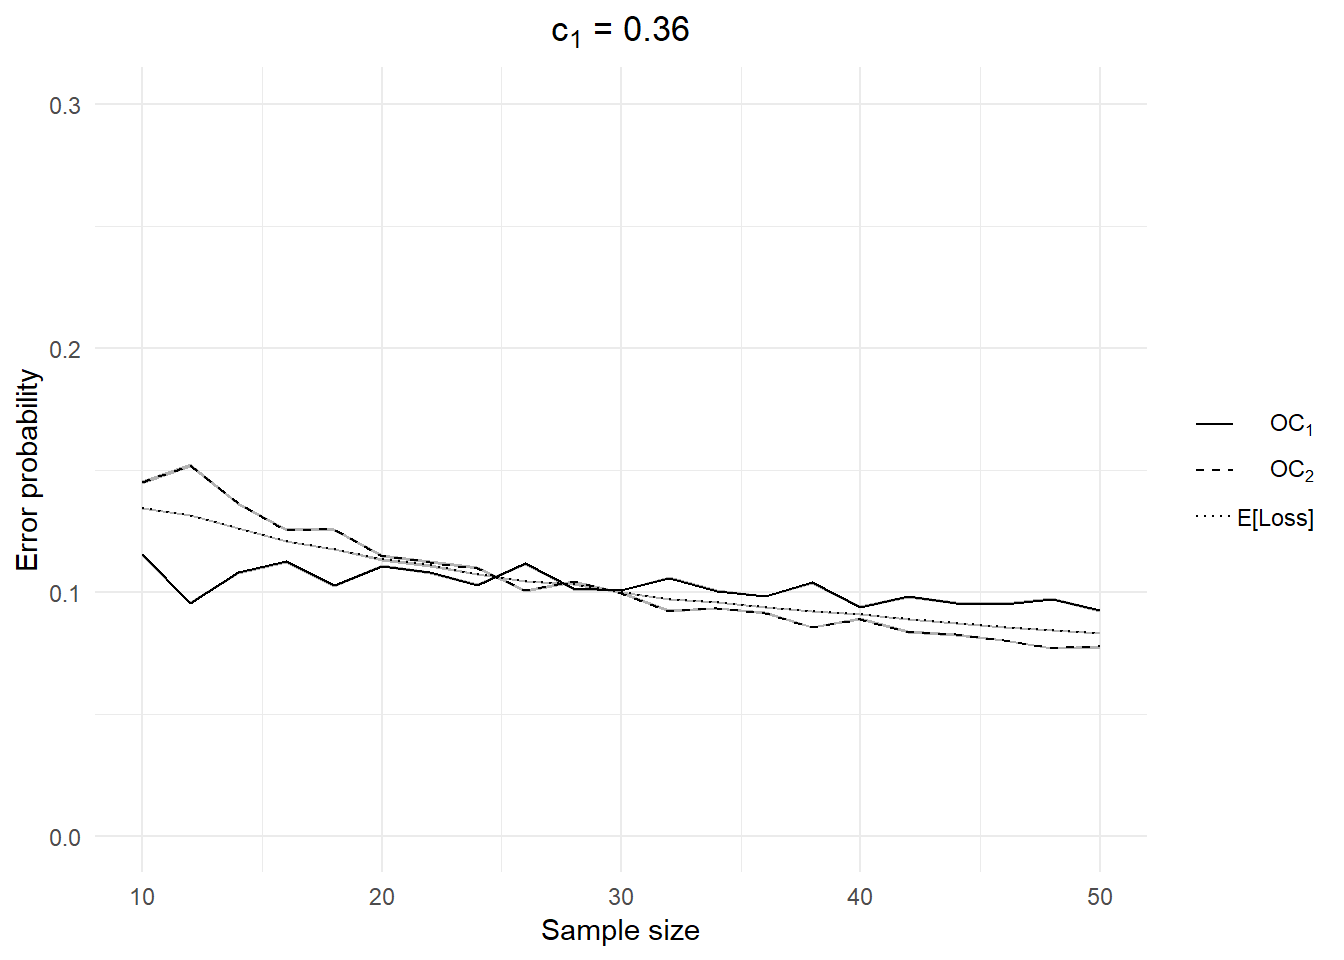
\includegraphics[width=0.9\linewidth,height=0.7\textheight]{Bayes_pilot_pres_files/figure-beamer/unnamed-chunk-7-1}

\end{frame}

\hypertarget{discussion}{%
\section{Discussion}\label{discussion}}

\begin{frame}{Implications}
\protect\hypertarget{implications}{}

Need to think more carefully about progression criteria and what they
are designed to do

Likewise, rules-of-thumb for sample size should be used with caution

Pilot trials can realiably distinguish between feasible and infeasible
cases with typical pilot sample sizes, if we evaluate from the
perspective of a subjective prior belief

We can start assessing effectivenss using this approach, and thus avoid
many futile definitive trials

\end{frame}

\begin{frame}{Limitations}
\protect\hypertarget{limitations}{}

Need a lot of extra input from the people designing the trial -
hypotheses and priors

Computation is slow when out of a conjugate setting - makes sample size
choice difficult to evaluate

Pre-specifying an amber region might be difficult (but note flexibility
to change once results are seen)

Piecewise constant loss function keeps things simple, but is unrealistic

\end{frame}

\begin{frame}{References}
\protect\hypertarget{references}{}

\end{frame}

\hypertarget{supplemenatary-material}{%
\section{Supplemenatary material}\label{supplemenatary-material}}

\begin{frame}{Loss parameters and OCs}
\protect\hypertarget{loss-parameters-and-ocs}{}

Figure

\end{frame}

\begin{frame}{Sample size}
\protect\hypertarget{sample-size}{}

Figure

\end{frame}

\begin{frame}{TIGA-CUB OCs}
\protect\hypertarget{tiga-cub-ocs}{}

Figure

\end{frame}

\begin{frame}{TIGA-CUB sample size}
\protect\hypertarget{tiga-cub-sample-size}{}

Figure

\hypertarget{refs}{}
\leavevmode\hypertarget{ref-Avery2017}{}%
Avery, Kerry N L, Paula R Williamson, Carrol Gamble, Elaine O'Connell
Francischetto, Chris Metcalfe, Peter Davidson, Hywel Williams, and Jane
M Blazeby. 2017. ``Informing Efficient Randomised Controlled Trials:
Exploration of Challenges in Developing Progression Criteria for
Internal Pilot Studies.'' \emph{BMJ Open} 7 (2): e013537.
\url{https://doi.org/10.1136/bmjopen-2016-013537}.

\leavevmode\hypertarget{ref-Eldridge2015}{}%
Eldridge, Sandra M, Ceire E Costelloe, Brennan C Kahan, Gillian A
Lancaster, and Sally M Kerry. 2015. ``How Big Should the Pilot Study for
My Cluster Randomised Trial Be?'' \emph{Statistical Methods in Medical
Research}. \url{https://doi.org/10.1177/0962280215588242}.

\leavevmode\hypertarget{ref-Eldridge2016}{}%
Eldridge, Sandra M., Gillian A. Lancaster, Michael J. Campbell, Lehana
Thabane, Sally Hopewell, Claire L. Coleman, and Christine M. Bond. 2016.
``Defining Feasibility and Pilot Studies in Preparation for Randomised
Controlled Trials: Development of a Conceptual Framework.'' Edited by
Chiara Lazzeri. \emph{PLOS ONE} 11 (3): e0150205.
\url{https://doi.org/10.1371/journal.pone.0150205}.

\leavevmode\hypertarget{ref-Hampson2017}{}%
Hampson, Lisa V, Paula R Williamson, Martin J Wilby, and Thomas Jaki.
2017. ``A Framework for Prospectively Defining Progression Rules for
Internal Pilot Studies Monitoring Recruitment.'' \emph{Statistical
Methods in Medical Research} 0 (0): 0962280217708906.
\url{https://doi.org/10.1177/0962280217708906}.

\end{frame}

\end{document}
